\lstset{language=Matlab}
\lstset{frame=single}
\section{Matlab}
\subsection{Pre-processing}
Before any objects in our image can be detected as a circle, the image has to be processed in different ways. Each step is described below.

\subsubsection{Normalize color-values}
The example pictures has different lightening conditions, one of them e.g., has subtile shadows along the edges of the sweets, the others don't. Most of the sweets in the pictures have shadow on themselves. This often becomes a problem when we try to separate the colored sweets from each other. The way to get around this problem is to normalize the colors as a step before the color separation process. For each color plane, R, G, B, we divide the color-values by the magnitude of the combined R,G,B vector:
\\
\lstinputlisting[firstline=4, lastline=6]{../matlab/normalizeColorValues.m}
\mbox{}\\
This is resulting in the following image:
\\
\centerline{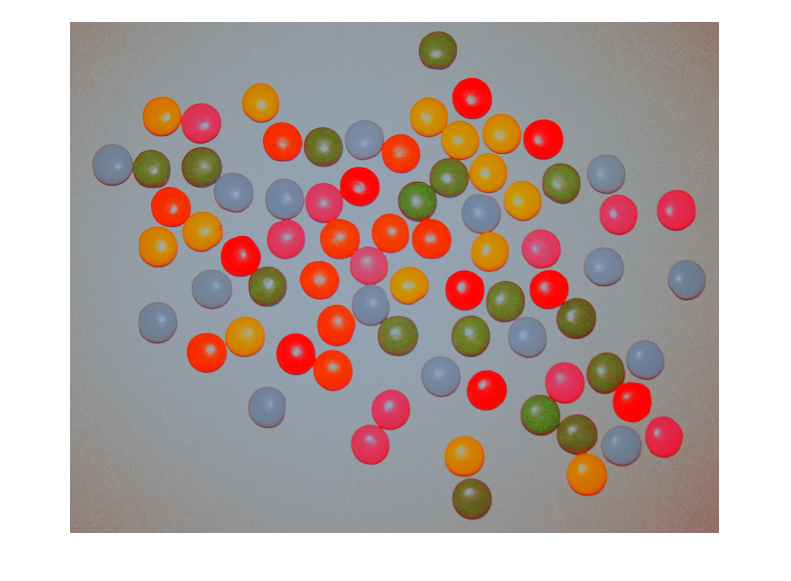
\includegraphics[scale=0.3]{../results/sweetsA03_normalized_colors.png}}
\mbox{}\\
\subsubsection{Separating colors}
SeparateColors.m function is used to filter out the different colors. It takes in a multi-color-image matrix, and returns six images. Each image contains only the non-stops of a certain color. The images are generated by subtracting the unwanted colors, and increasing the values of the wanted colors.

For example: The blue non-stops are separated by subtracting the green-image from the blue-image, thus removing green nonstops. 
\\
\centerline{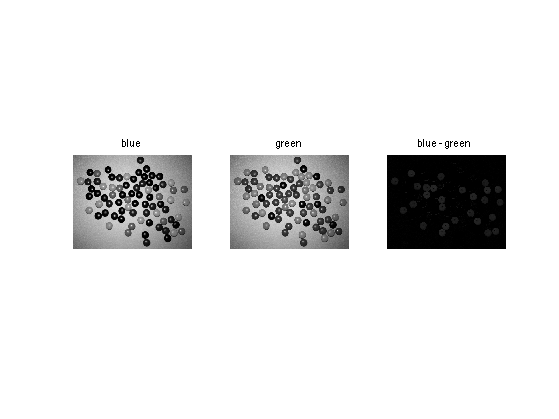
\includegraphics[clip=true, trim=40 100 40 80]{separate_step1.png}}
\\*
As the green and the blue images look quite alike, the resulting image is mostly black. To be able to further subtract colors from the image, the max values are increased. Red colors are then subtracted from the image.
\\
\centerline{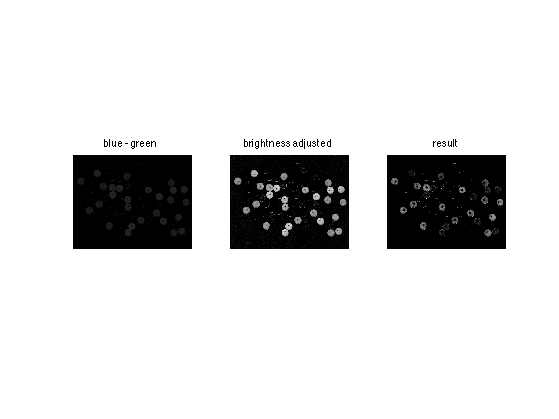
\includegraphics[clip=true, trim=40 100 40 80]{separate_step2_1.png}}
\mbox{}
Below is the code that generated the resulting image. 
\lstinputlisting[firstline=22, lastline=28]{../matlab/separateColors.m}
\mbox{}\\
The image created so far has the blue objects represented as the brightest circles. To remove the unwanted representation of other objects, thresholding is used.

After the thresholding process the image has blobs of pixels, but because of the highlight created by the flashlight, we get holes inside our thresholded sweets. The holes are therefore filled with a inbuilt matlab function, \emph{imfill(image, type)},
\\
\lstinputlisting[firstline=80, lastline=80]{../matlab/separateColors.m}
\mbox{}\\
To remove noise from the images, the images are median filtered. This is done by the function \emph{medianFilter(img, filterSize)}. 
\\
\lstinputlisting{../matlab/medianFilter.m}

\centerline{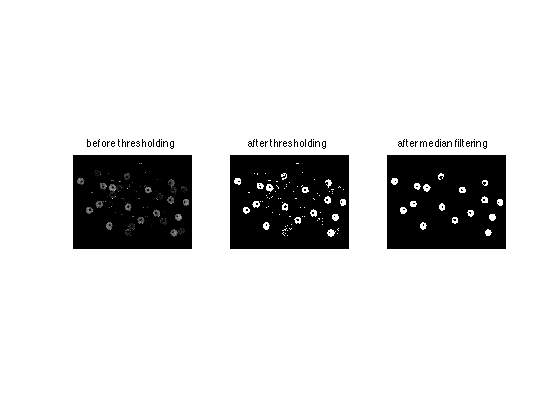
\includegraphics[clip=true, trim=40 100 40 80]{separate_step3_1.png}}

Even though the colors now are separated, the binary shape of the sweets is uneven and some of the sweets look like a circle with waves on it. Some of the sweets is therefore hard to detect as circles, as is. This uneveness is resolved by executing a sequence of open and closing filters, with a disk filter,
\\
\lstinputlisting[firstline=3, lastline=6]{../matlab/openAndClose.m}
\mbox{}\\
After all these steps, the final bit-mask will look like this:
\\ \newline
\centerline{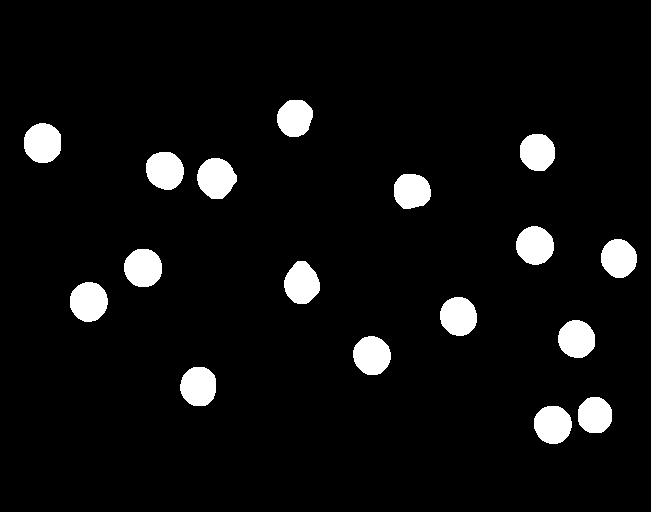
\includegraphics[scale=0.3]{../results/sweetsA03_blue_sweets.png}}
\mbox{}\\
\subsection{Circle detection and localization}
Now that the colored sweets are separated and represented as circular binary objects, the detection of the sweets' centroid and radius can be detected. We tried to implement our own circle detector, but that's before we heard that we - for this particular project - could use the inbuilt matlab function \emph{imfindcircles(img, [radmin, radmax])}. Since we implemented some parts of this circular detection system, we will describe how and why we tried this approach. To understand how the canny edge detector and the hough transform worked, we read some papers \cite{canny1,hough1} that is also the basis of our implementation.
\subsubsection{Canny edge-detector}
Canny edge detector takes an image and finds the edges based on the gradients found in the image. It also finds the direction of the edges and their magnitude. All this information is passed on to the hough algorithm later on. The gradients is found by convolving the image with a sobel operator,
\\
\lstinputlisting[firstline=2, lastline=10]{../matlab/findGradients.m}
\mbox{}\\
The magnitude and angle (theta) is calculated for each edge,
\\
\lstinputlisting[firstline=20, lastline=23]{../matlab/edgeCanny.m}
\mbox{}\\
Now, all those angles has to be detected by their direction in a 8-connected neighbour fashion, and the edges has to be stripped down, so the maximum edge value is preserved, while the other less-valued edge values is thrown away. Next step, the image is thresholded, so the hard edges and soft edges is separated. We then want to find pixels which has low values that's connected to a pixel with a high value, to extend the edges in our edge map. This process is called hysteresis. Now we have a complete edge map, as seen below. For more insight in this process, see \emph{edgeCanny.m}.
\\
\centerline{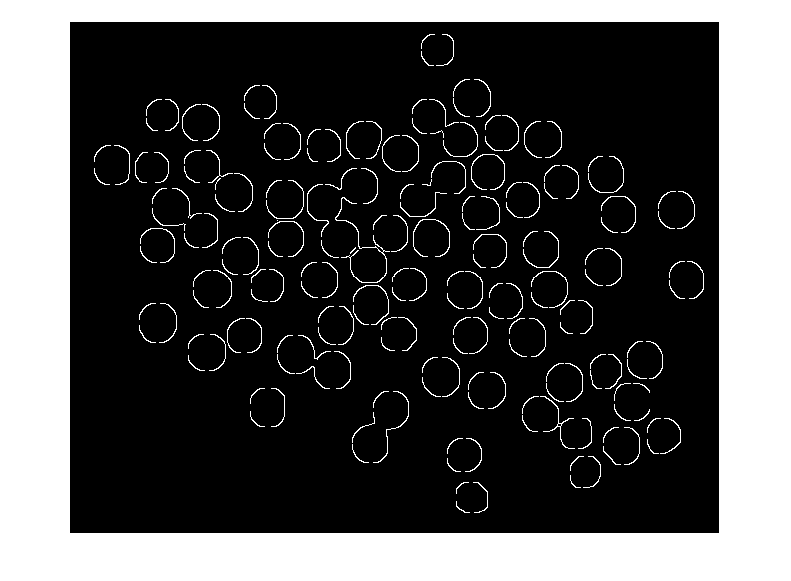
\includegraphics[scale=0.3]{../results/sweetsA03_edges.png}}
\subsubsection{Hough circular transform}
Now when the edges is detected, we can try detecting the centroids using a hough transform. 
\subsection{Improvements}
A more adjustable but computational heavier approach to separate colors in the image, is by filtering. Each matrix would then have to be filtered, to extract the r, g and b values. An appropriate range would have to be set, for this method to work. For example: The blue non-stops in a image would be separated by filtering the values 0 to 50 from the red matrix, 0 to 50 from the green matrix and 205 to 255 from the blue image. A new matrix is then generated. The overlapping values are represented as 1.0 in the new matrix. The remaining values are set to 0.0. \\

